\section{Introduction}
\label{sec:intro}

\begin{figure}[t]
  \centering
  % figures/fig1_teaser.pdf = rsvg-convert of figures/fig1_teaser.svg (pdflatex cannot read SVG); source: draw/
  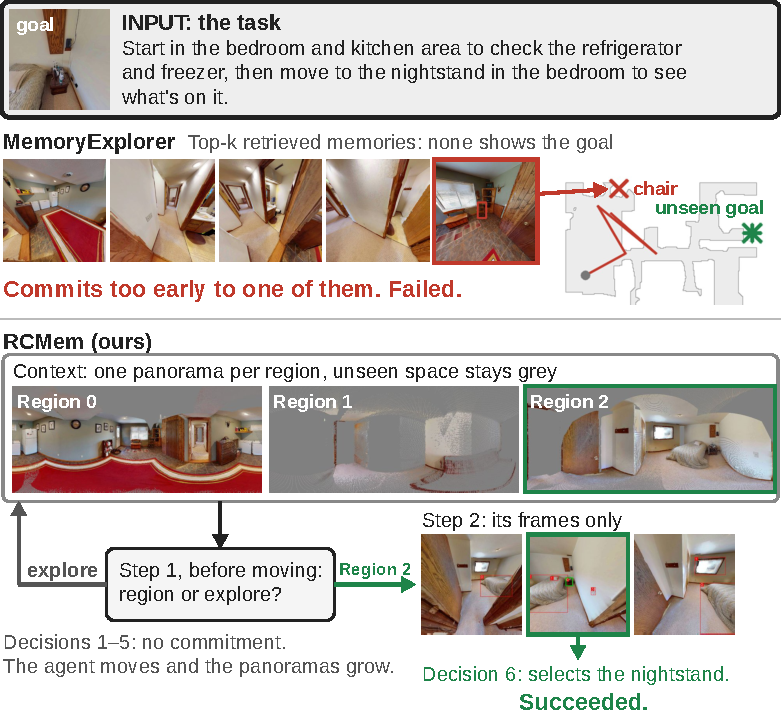
\includegraphics[width=\linewidth]{figures/fig1_teaser}
  % Real subtask 00877-4ok3usBNeis_0_2. RCMem panel: zero-shot RPcu run, whose prompts also held close-ups.
  \caption{\textbf{Commit or explore.} On this LMEE-Bench subtask,
  MemoryExplorer retrieves five memories, none showing the goal, and commits to
  one of them, a chair in another room, before the goal's room has been
  observed (top; map: its path). \ours{} keeps one panorama per region in the
  VLM's context, leaves unobserved space visible, and loops, choosing a region
  before choosing a target and before moving, until it finds the goal (bottom).
  Context shown as at the last decision; frontier views are not shown.}
  \label{fig:teaser}
\end{figure}

An embodied agent asked to ``check the Christmas tree and the dryer, then the
bedroom nightstand'' must explore an unfamiliar home, remember what it sees,
and, for each subtask, decide again and again whether the goal is already in
its memory. If it is, the agent should \emph{commit}: travel to the remembered
object. If it is not, it should \emph{explore}. A wrong commitment costs a
wasted trip and often the subtask; a needless exploration costs only steps.
Every memory-based agent faces this decision, whatever form its memory takes,
and in multi-goal tasks it faces it at nearly every step
(\cref{fig:teaser}).

Work on embodied memory has mostly improved \emph{what} is remembered and
\emph{how} it is found. Explicit memories store views, graphs or 3D maps
outside the model and retrieve from them: multi-view snapshots~\cite{3dmem},
RL-trained retrieval~\cite{lmee}, room-level graphs~\cite{stegnav,evomemnav}
and 3D Gaussian maps~\cite{gsmem,lagmemo}. Implicit memories keep the history in
the policy's own context and compress it to fit: StreamVLN~\cite{streamvln}
prunes its KV cache in 3D, JanusVLN~\cite{janusvln} keeps separate spatial and
semantic caches, and AstraNav-Memory~\cite{astranav} spends about 30 tokens per
image. Where the question of \emph{when} to trust memory is addressed, it is
mostly handled after the agent has travelled: the target is verified on
arrival~\cite{stegnav,evomemnav}, checked against the expected
room~\cite{contextnav}, or re-rendered and checked again~\cite{3dgsnav}. The
closest exception is EvoMemNav~\cite{evomemnav}, where a low-confidence anchor
choice sends the agent back to exploring. We know of no method that decides,
before moving and from what each region has and has not shown, whether the goal
could be in memory yet.

\paragraph{Where a memory agent fails.}
We take MemoryExplorer~\cite{lmee}, a Qwen2.5-VL-7B~\cite{qwen25vl}
agent trained with GRPO to retrieve from a CLIP-indexed memory bank, run it on
LMEE-Bench~\cite{lmee} in HM3D-Sem scenes~\cite{hm3dsem}, and label every
commitment with simulator ground truth: regions, instances and their
visibility. Retrieval is not the bottleneck. The correct memory is among the
retrieved candidates in 84--91\% of decisions, and only 2 of 145 questions need
more than one stored view. The commitment is. On the full benchmark (one run),
57.4\% of the 625 navigation failures are commitments to the wrong remembered
object, and 272 of these 359 were made before the goal had been seen at all; on
a 58-task subset, 87.5\% of same-category distractor choices and 97.4\% of other
premature choices lie in a region other than the goal's. The agent is, in
effect, blind until it has seen the goal's region. On the full benchmark, once
that region has been observed, it commits far more often when the goal is in
memory than when it is not (41.5\% vs.\ 19.0\% of decisions); before, it commits
as often either way (24.4\% vs.\ 26.7\%), and 57\% of all decisions are made in
this state.

\paragraph{The decision must come before moving.}
With ground-truth regions, restricting commitments to the goal's region before
the agent travels raises the success rate (SR) from 25.9 to 41.7 and cuts
premature commitments from 28.9\% to 1.8\% (58-task subset, three seeds; we
treat differences below 5.1~SR, twice the pooled run-to-run standard deviation,
as noise). The
remedies used in the field do much less. Naming the goal's region in the prompt
adds 3.4~SR and verifying the target on arrival 4.9~SR (single runs against
the baseline before our orientation fix), although the verifier's
rejections are correct 95.1\% of the time: after a correct rejection, the agent
commits to the next wrong object, and for most wrong commitments there was
nothing right to verify yet. The oracle gate is a ceiling, not a method; the
question is what an agent needs in order to make the same decision itself.

\paragraph{Where the structure should live.}
Keeping the whole episode in the model's context, as implicit memories do,
seems a natural answer: nothing can be lost to retrieval, and a stream of views
pruned by 3D novelty keeps the goal view in 95.5\% of decisions within 16k
tokens. Holding the model fixed, we find the opposite. Without structure, the
context shows the agent every distractor at once: SR falls to 19.6, from 25.9
with the retrieved bank, and premature commitments rise to 40.6\%. Restricting
the same context to the goal's region lifts SR to 37.6 and removes nearly all
premature commitments (1.3\%), a gain of 18.0~SR over the unstructured
context, on a par with the 15.8~SR the same gate adds to the bank (the
difference is within noise). Knowing only the
region's \emph{type} recovers about half of this gain (52\%); with the bank,
a third of the type gate's remaining wrong commitments land in a second room
of the same type and 38\% in rooms that no label covered. Implicit memory lacks
structure, not capacity, and the structure it needs is region
\emph{instances}, not region names.

\paragraph{\ours.}
We propose \ours{} (Region-scoped Context Memory), a VLM whose context is its
memory, organised by region. Observations are pruned by 3D novelty and assigned
to regions segmented from the free-space map at narrow
passages~\cite{bormann2016room}. Each region enters the context as one
equirectangular panorama rendered from the point that sees most of it. Pixels
that nothing has observed stay grey, so the model sees both what a region
contains and how much of it is still unseen, which is exactly the blind state
above. Regions carry no labels: whether a region is the bedroom a subtask
refers to is read from its pixels. At each decision the agent commits in two
steps before it moves. From the panoramas, the subtask markers and one view per
frontier, it chooses a region or to explore; then, from that region's kept
frames only, it selects the goal or declines.
% If the frozen zero-shot config (RPcu) stays the main one, add its room
% close-ups here, e.g. ``with a few close-up views of each region''.
Subtask markers and the order of the region blocks carry time.
\ours{} is fine-tuned on context streams rebuilt from training trajectories
without hand-inserted goal views, including absent-goal and distractor streams
in which exploring is the right answer, and with an objective that charges a
wrong commitment more than a needless exploration. Outside the model it stores
the pruned RGB-D frames, their camera poses and the floor map. There is
no retrieval index and no stored feature, and a decision takes at most two VLM
calls.

% Dev reference (P3, subset, seed 77, zero-shot, Qwen3-VL-8B; not main results):
% F1 31.2, RCMem RP 34.6, RPcu 38.6 SR.
We evaluate on the full LMEE-Bench (166 tasks, three seeds) and on
GOAT-Bench~\cite{goatbench}. \ours{} runs on Qwen3-VL-8B~\cite{qwen3vl}; because
MemoryExplorer uses Qwen2.5-VL-7B, the backbone's own gain is reported
separately. Moving the context without
regions from Qwen2.5-VL-7B to Qwen3-VL-8B gives \tbd{+X}~SR, and \ours{} adds
\tbd{+Y}~SR over it on the same model. Premature commitments fall from
\tbd{X}\% to \tbd{Y}\%, and \ours{} stores \tbd{X}\,MB per episode against
\tbd{Y}\,MB. Our diagnosis uses one agent with two memory designs, a retrieved
bank and an in-context stream, on one benchmark; we evaluate the method on two.

\noindent In summary, we make four contributions:
\begin{enumerate}
  \setlength{\itemsep}{1pt}
  \item \textbf{A ground-truth diagnosis of memory failures.} We show that a
    strong memory agent fails at the commitment, not at retrieval: most wrong
    commitments are made before the goal's region has been observed, and in
    that state the agent cannot tell whether the goal is in memory.
  \item \textbf{In-context memory needs structure.} With the model held fixed,
    an unstructured context is worse than a retrieved bank, while scoping it to
    the goal's region gains as much as the same gate gives the bank; region
    types alone recover only about half of this gain.
  \item \textbf{\ours.} A context memory with one panorama per region that
    shows unobserved space, a two-step commitment made before moving, and
    training on streams where the goal is often absent. It is compact and
    direct: no retrieval, no stored features, at most two VLM calls per
    decision.
  \item \textbf{A sound evaluation.} We fix a start-orientation bug that
    affected every LMEE episode we ran, set a noise band from repeated baseline runs,
    correct QA accuracy for an answer-letter prior (always answering ``B''
    scores 59.3\%), and separate the backbone's gain from the method's with
    same-backbone controls.
\end{enumerate}
